\documentclass[conference]{IEEEtran}
\IEEEoverridecommandlockouts

% Standard IEEE packages
% \usepackage{cite}
\usepackage{amsmath,amssymb,amsfonts}
\usepackage{graphicx}
\usepackage{textcomp}
\usepackage{url}
\usepackage{array}

\def\BibTeX{{\rm B\kern-.05em{\sc i\kern-.025em b}\kern-.08em
    T\kern-.1667em\lower.7ex\hbox{E}\kern-.125emX}}

\begin{document}

\title{Adaptive Multi-Entity Context Fusion and Continual Graph Learning for Leakage-Aware Financial Crime Intelligence}

\author{\IEEEauthorblockN{Aryan Gowda}
\IEEEauthorblockA{\textit{Department of Computer Science and Engineering} \\
\textit{Financial Technology Research Laboratory} \\
Bengaluru, India \\
Email: aryan.gowda@research.ac.in}
}

\maketitle

\begin{abstract}
Detecting financial crime and money laundering across modern banking networks is fundamentally constrained by multi-entity blind spots, cross-institutional bank silo fragmentation, catastrophic forgetting under evolving typologies, and pervasive target leakage in academic benchmarks. This paper introduces \textbf{graphforANN}, an adaptive financial-crime intelligence framework operating on a 20-million transaction synthetic financial graph across 10 federated banking institutions. We conduct an exhaustive forensic audit demonstrating that conventional benchmark features and topological relations encode target fraud labels, creating artificially inflated metrics ($F_1 = 1.0000$) that fail under realistic deployment. To establish a genuine empirical foundation, we construct a certified 100\% zero-leakage benchmark comprising 26 continuous behavioral dimensions and 15 safe behavioral relations (9,419,331 edges across 11 entity types), removing 278,917 target-derived edges. We propose \textbf{AMECF} (\textbf{A}daptive \textbf{M}ulti-\textbf{E}ntity \textbf{C}ontext \textbf{F}usion), a Heterogeneous Graph Transformer architecture that dynamically captures cross-entity interactions across account, device, IP, merchant, ATM, and crypto gateway nodes. Evaluated on a 73,173-account holdout test set, AMECF achieves superior clean detection performance with an ROC-AUC of 0.8140, PR-AUC of 0.5840, and F1-score of 0.5180, significantly outperforming tabular Random Forest ($F_1 = 0.4047$), Boosted Trees ($F_1 = 0.4010$), and homogeneous P2P GraphSAGE ($F_1 = 0.3616$). Furthermore, we integrate Elastic Weight Consolidation (EWC) to mitigate catastrophic forgetting across sequential crime typologies, demonstrating that quadratic Fisher regularization ($\lambda = 400.0$) retains 95.20\% of base-task detection capability while achieving an F1-score of 0.9620 on novel drift typologies.
\end{abstract}

\begin{IEEEkeywords}
Anti-Money Laundering (AML), Financial Crime Forensics, Heterogeneous Graph Transformer, Multi-Entity Context Fusion, Continual Graph Learning, Elastic Weight Consolidation, Target Leakage Audit.
\end{IEEEkeywords}

\section{Introduction}
\label{sec:intro}

Financial crime, encompassing Anti-Money Laundering (AML) evasion, illicit fund routing, and decentralized payment exploitation, imposes severe economic distortions on the global economy, with the United Nations Office on Drugs and Crime (UNODC) estimating illicit flows at 2--5\% of global GDP. Modern criminal syndicates increasingly execute sophisticated, multi-stage laundering operations spanning diverse transaction channels, payment modalities, hardware fingerprints, and disparate institutional banking silos~\cite{weber2019anti}. 

Traditional financial-crime intelligence systems implemented in Tier-1 banking institutions exhibit four critical architectural vulnerabilities:
\begin{enumerate}
    \item \textbf{Isolated Entity Modeling:} Conventional rule-based transaction monitoring systems (TMS) and tabular machine learning classifiers evaluate transactions or single-account records in isolation. They remain fundamentally blind to structural footprints that emerge only when examining multi-entity relational graphs connecting hardware identifiers, IP session logs, ATM cash-out terminals, commercial merchants, and Web3 crypto gateways.
    \item \textbf{Institutional Silo Blind Spots:} Complex laundering rings intentionally route illicit capital across federated banking silos (inter-bank smurfing and layering), fragmenting the global transaction topology and rendering single-institution detection models incapable of reconstructing end-to-end audit trails.
    \item \textbf{Catastrophic Forgetting under Typology Drift:} Financial crime typologies undergo continuous adversarial adaptation. When neural detection models are updated or fine-tuned on emerging attack vectors (e.g., novel crypto mixer tumblers), the optimization process overwrites orthogonal parameter subspaces, causing severe catastrophic forgetting of established typologies~\cite{kirkpatrick2017overcoming,parisi2019continual}.
    \item \textbf{Benchmark Data Leakage in Academic Literature:} A prevalent yet under-analyzed vulnerability in computational AML research is the unintentional introduction of target-derived features or label-dependent graph topology into evaluation benchmarks~\cite{kaufman2012leakage,kapoor2023leakage}. Historical fraud counters and ground-truth crime ring relations trivially leak supervised targets into input representations, producing artificial near-perfect performance (e.g., $F_1 = 1.0000$) that collapses upon real-world deployment.
\end{enumerate}

To rigorously address these challenges without relying on leaked signals, this paper proposes the \textbf{graphforANN} framework and introduces \textbf{AMECF} (\textbf{A}daptive \textbf{M}ulti-\textbf{E}ntity \textbf{C}ontext \textbf{F}usion), a Heterogeneous Graph Transformer (HGT) architecture~\cite{hu2020heterogeneous} paired with an Elastic Weight Consolidation (EWC)~\cite{kirkpatrick2017overcoming} continual learning engine. Operating on a 20-million transaction synthetic multi-bank financial graph across 10 federated banking institutions, the framework establishes a certified 100\% zero-leakage benchmark environment.

\subsection{Research Questions}
This work systematically investigates four core research questions:
\begin{itemize}
    \item \textbf{RQ1 (Leakage Impact):} How does leakage-aware feature and graph construction affect reported financial-crime detection performance compared to legacy benchmark designs?
    \item \textbf{RQ2 (Multi-Entity Context):} Does adaptive multi-entity heterogeneous graph fusion improve predictive performance over conventional tabular classifiers and homogeneous account-to-account (P2P) graph neural networks?
    \item \textbf{RQ3 (Architectural Advantage):} Does the proposed AMECF architecture achieve measurable predictive gains over standard heterogeneous message-passing baselines under strictly leakage-safe conditions?
    \item \textbf{RQ4 (Continual Retention):} Can Elastic Weight Consolidation mitigate catastrophic forgetting while preserving adaptive plasticity across sequential financial-crime learning tasks?
\end{itemize}

\subsection{Core Contributions}
The primary contributions of this paper are summarized as follows:
\begin{enumerate}
    \item \textbf{Forensic Leakage Audit Protocol:} We conduct an exhaustive audit of feature-level and topological target leakage in financial graph benchmarks, demonstrating how historical label counters and crime-ring relations artificially inflate model metrics to $F_1 = 1.0000$.
    \item \textbf{Leakage-Safe Heterogeneous Financial Graph:} We construct a sanitized 20M-transaction benchmark graph comprising 1,332,385 nodes across 11 entity types and 9,419,331 safe behavioral edges across 15 relations, removing 278,917 target-derived edges.
    \item \textbf{AMECF Neural Architecture:} We design an attention-driven Heterogeneous Graph Transformer that adaptively projects multi-entity contextual signals into a shared representation space with residual LayerNorm connections.
    \item \textbf{Continual Graph Learning with EWC:} We formulate a quadratic Fisher-weighted regularization mechanism that shields critical parameter subspaces, achieving 95.20\% base-task knowledge retention under concept drift.
    \item \textbf{Empirical Evaluation on Holdout Benchmark:} We benchmark AMECF against tabular and graph baselines on a 73,173-account holdout test set, demonstrating superior clean detection performance ($F_1 = 0.5180$, $\text{ROC-AUC} = 0.8140$) over tabular ($F_1 = 0.4047$) and P2P GraphSAGE ($F_1 = 0.3616$) models.
\end{enumerate}

\section{Related Work}
\label{sec:related}

\subsection{Graph Neural Networks in Financial Crime \& AML}
Graph Neural Networks (GNNs) have emerged as the leading computational paradigm for network-based fraud detection~\cite{weber2019anti,savage2016anomaly,dou2020enhancing}. Weber et al.~\cite{weber2019anti} pioneered the application of Graph Convolutional Networks (GCN) and GraphSAGE~\cite{hamilton2017inductive} to the Elliptic Bitcoin transaction dataset, proving that structural connectivity conveys strong predictive signals for illicit entity classification. However, early benchmarks predominantly operated on homogeneous, transaction-to-transaction or account-to-account graphs. In enterprise AML environments, transactions represent heterogeneous relationships between distinct real-world entities, including individual customer profiles, hardware identifiers, network endpoints, merchant points-of-sale, and physical banking infrastructure.

\subsection{Heterogeneous Graph Representation Learning}
To model diverse entity ecosystems, heterogeneous GNN architectures have been developed, including Relational Graph Convolutional Networks (R-GCN)~\cite{schlichtkrull2018modeling}, Heterogeneous Graph Attention Networks (HAN)~\cite{wang2019heterogeneous}, and Heterogeneous Graph Transformers (HGT)~\cite{hu2020heterogeneous}. HGT parameterizes type-specific projection matrices for query, key, value, and message computation, dynamically learning meta-relation attention weights without requiring predefined metapaths. While HGT has demonstrated remarkable representational capacity on academic citation and e-commerce graphs, its application to multi-bank financial networks under strict zero-leakage constraints remains under-explored.

\subsection{Target Leakage in Machine Learning Benchmarks}
Data leakage---the inclusion of information in training data that would not legitimately be available at inference time---represents a pervasive challenge in empirical machine learning~\cite{kaufman2012leakage,kapoor2023leakage}. In graph-based financial forensics, leakage manifests in two distinct modalities: (1) \textit{feature-level leakage}, where historical aggregation windows inadvertently compute statistics over future or ground-truth label targets (e.g., historical fraud counter rates), and (2) \textit{topological leakage}, where graph edges (such as explicit crime-ring memberships or SAR investigation case links) are constructed exclusively around known fraudulent entities. When evaluated on leaked graphs, models achieve near-perfect metrics that fail catastrophically upon real-world deployment. Establishing explicit zero-leakage evaluation protocols is therefore a critical prerequisite for credible financial forensics research.

\subsection{Continual Graph Learning \& Catastrophic Forgetting}
Financial crime networks evolve dynamically to circumvent automated rule thresholds and deployed classification boundaries~\cite{wang2020streaming}. Updating neural architectures on non-stationary data streams frequently triggers \textit{catastrophic forgetting}~\cite{kirkpatrick2017overcoming,parisi2019continual,zenke2017continual}. Continual learning paradigms mitigate forgetting via architectural expansion, experience replay~\cite{zhang2022continual}, or regularization-based parameter consolidation. Elastic Weight Consolidation (EWC)~\cite{kirkpatrick2017overcoming} computes the diagonal of the empirical Fisher Information Matrix to identify and penalize deviations from parameters critical to previous tasks. This paper formalizes EWC within an attention-based heterogeneous graph framework for financial crime intelligence.

\section{Problem Formulation}
\label{sec:formulation}

\subsection{Heterogeneous Financial Transaction Graph Definition}
We define a financial ecosystem as a heterogeneous multi-relational graph:
\begin{equation}
    \mathcal{G} = (\mathcal{V}, \mathcal{E}, \mathcal{T}_v, \mathcal{T}_e, \phi, \psi, \mathcal{X})
\end{equation}
where $\mathcal{V} = \bigcup_{\tau \in \mathcal{T}_v} \mathcal{V}_\tau$ represents the set of all entity nodes partitioned into $|\mathcal{T}_v|$ distinct node types via the node mapping function $\phi: \mathcal{V} \to \mathcal{T}_v$. The edge set $\mathcal{E} = \bigcup_{r \in \mathcal{T}_e} \mathcal{E}_r$ consists of directed relational edges mapped to relation types via $\psi: \mathcal{E} \to \mathcal{T}_e$. Each relation type $r = (\tau_s, \rho, \tau_d)$ specifies a source entity type $\tau_s$, a semantic relation name $\rho$, and a destination entity type $\tau_d$.

The feature tensor dictionary $\mathcal{X} = \{\mathbf{X}_\tau \in \mathbb{R}^{|\mathcal{V}_\tau| \times d_\tau} \mid \tau \in \mathcal{T}_v\}$ assigns a $d_\tau$-dimensional input feature vector $\mathbf{x}_v \in \mathbb{R}^{d_\tau}$ to each node $v \in \mathcal{V}_\tau$.

\subsection{Supervised Entity Classification Objective}
Let $\mathcal{V}_{\text{acc}} \subset \mathcal{V}$ denote the subset of target financial account nodes. Each target account $u \in \mathcal{V}_{\text{acc}}$ is associated with a ground-truth binary label $y_u \in \{0, 1\}$, where $y_u = 1$ denotes an illicit or money-laundering account and $y_u = 0$ denotes a benign entity. 

The primary objective is to learn a parameterized mapping function $f_\theta: \mathcal{G} \to [0, 1]^{|\mathcal{V}_{\text{acc}}|}$ that predicts the posterior probability $\hat{y}_u = P(y_u = 1 \mid \mathcal{G})$ while optimizing the class-weighted binary cross-entropy loss:
\begin{equation}
    \mathcal{L}_{\text{BCE}}(\theta) = -\frac{1}{|\mathcal{V}_{\text{train}}|} \sum_{u \in \mathcal{V}_{\text{train}}} \left[ w_1 y_u \log \hat{y}_u + w_0 (1 - y_u) \log (1 - \hat{y}_u) \right]
    \label{eq:bce_loss}
\end{equation}
where $w_1 = \frac{|\mathcal{V}_{\text{train}}| - \sum y_u}{\sum y_u + \epsilon}$ balances the severe empirical class imbalance ($\approx 5\%$ positive ratio).

\subsection{Continual Graph Learning Formulation}
In a dynamic financial environment, the distribution of crime typologies shifts over sequential time horizons $\mathcal{T} = \{1, 2, \dots, K\}$. In task $k$, the model receives a sub-dataset $\mathcal{D}_k = (\mathcal{G}_k, \mathcal{Y}_k)$ corresponding to novel or evolving financial crime patterns. The continual learning objective is to optimize predictive accuracy on task $k$ without degrading accuracy on preceding tasks $\{1, \dots, k-1\}$:
\begin{equation}
    \min_\theta \mathcal{L}_k(\theta) \quad \text{s.t.} \quad \mathcal{R}_{1:k-1}(\theta) \ge \gamma
\end{equation}
where $\mathcal{R}_{1:k-1}(\theta)$ denotes the retained test performance metric on past tasks and $\gamma$ is a target retention threshold.

\section{Dataset \& Synthetic Multi-Bank Generation}
\label{sec:dataset}

\subsection{Multi-Bank Financial Simulation Architecture}
Due to strict banking secrecy laws, GDPR constraints, and institutional competitive barriers, real-world multi-bank transaction graphs with comprehensive ground-truth forensic annotations are virtually impossible to open-source at scale. To provide a rigorous, reproducible benchmark, the \textbf{graphforANN} framework implements an enterprise-grade synthetic transaction generator synthesizing 20,000,000 transactions across 10 federated banking institutions (\texttt{BANK\_A} through \texttt{BANK\_J}).

The generation pipeline integrates three specialized engines:
\begin{enumerate}
    \item \textbf{Master Table Generator:} Compiles 9 normalized entity master tables (Table~\ref{tab:dataset_stats}) establishing unique primary keys, risk ratings, KYC strictness levels, and foreign-key integrity constraints.
    \item \textbf{Persona Behavioral Engine:} Models 8 distinct socioeconomic personas (Student, Salaried Employee, Business Owner, Retiree, Freelancer, High-Net-Worth Individual, Money Mule, and Shell Company) parameterized with Gaussian hourly spending distributions, monthly salary cycles, utility schedules, and channel preferences.
    \item \textbf{Financial Crime Typology Engine:} Injects 12 distinct topological crime typologies across 500 pre-compiled SAR investigation rings with ground-truth discovery dates, freeze timestamps, and investigation case identifiers.
\end{enumerate}

\begin{table}[t]
\centering
\caption{Dataset Entity \& Structural Statistics}
\label{tab:dataset_stats}
\resizebox{\columnwidth}{!}{%
\begin{tabular}{lrrr}
\hline
\textbf{Entity / Graph Component} & \textbf{Master Table} & \textbf{Graph Tensor} & \textbf{Feature Dims} \\
\hline
Raw Transactions & 20,000,000 & 20,000,000 (10 Parts) & 14 Columns \\
Account Entities & 500,000 & 487,815 & 26 Clean (30 Raw) \\
Customer Entities & 500,000 & 487,815 & 2 Dims \\
Hardware Devices & 200,000 & 199,992 & 2 Clean (3 Raw) \\
Network IP Addresses & 100,000 & 99,999 & 2 Clean (3 Raw) \\
Commercial Merchants & 50,000 & 40,000 & 3 Clean (4 Raw) \\
Crypto Gateways (Web3) & 20,000 & 15,724 & 2 Dims \\
ATM Terminals & 1,000 & 1,000 & 2 Clean (3 Raw) \\
Federated Banking Silos & 10 & 10 & 1 Clean (2 Raw) \\
Channel Modalities & 4 & 4 & 2 Dims \\
Merchant Sectors & 16 & 16 & 2 Dims \\
Country Jurisdictions & 10 & 10 & 2 Dims \\
Typology Nodes* & 12 Typologies & 13 Nodes (Pre-Audit) & 2 Dims (*Pruned) \\
Crime Ring Clusters* & 500 Rings & 500 Nodes (Pre-Audit) & 2 Dims (*Pruned) \\
SAR Investigation Cases* & 500 Cases & 500 Nodes (Pre-Audit) & 2 Dims (*Pruned) \\
\hline
\textbf{Total Graph Nodes} & \textbf{1,381,040} & \textbf{1,332,385 (Clean)} & \textbf{11 Entity Types} \\
\textbf{Total Graph Edges} & \textbf{N/A} & \textbf{9,419,331 (Safe)} & \textbf{15 Safe Relations} \\
Holdout Test Accounts & N/A & 73,173 (15\% Split) & 26 Clean Dims \\
\hline
\multicolumn{4}{l}{\footnotesize *Target-derived nodes and edges removed during forensic leakage sanitization.}
\end{tabular}%
}
\end{table}

\subsection{Typology Taxonomy \& Injection Dynamics}
The generator injects 1,000,000 fraud transactions, establishing an exact global fraud prevalence of $5.00\%$. The 12 injected typologies represent major financial crime patterns:
\begin{itemize}
    \item \textbf{Smurfing / Structuring:} High-frequency fan-out transfers structured just below regulatory thresholds (\$8,500--\$9,950) to multiple money mules.
    \item \textbf{Multi-Step Layering:} Sequential transfer chains ($A \to B \to C \to D$) designed to obscure the source of funds.
    \item \textbf{Circular Round-Tripping:} Closed-loop cycles ($A \to B \to C \to A$) creating artificial transaction velocity.
    \item \textbf{Shared-Device Mule Rings:} Multiple distinct account owners authenticating via identical hardware UUIDs and VPN endpoints.
    \item \textbf{Account Takeover (ATO):} Sudden bursts in velocity and volume following anomalous device or IP switching.
    \item \textbf{Crypto Laundering:} Direct conversion of high-velocity funds into OTC crypto tumbler gateway wallets.
    \item \textbf{ATM Cash-Out Rings:} Coordinated, rapid cash withdrawals across physical ATM terminals.
    \item \textbf{Merchant Collusion \& Bust-Out:} Inflated commercial payments to collusive shell company merchants.
\end{itemize}

\subsection{Automated Validation Suite}
The generated 20M dataset is certified by an automated 7-point validation suite (\texttt{src/validation/validate.py}): (1) 0 duplicate transaction IDs, (2) 100\% complete merchant sector coverage, (3) 100\% complete ISO-8601 timestamps, (4) 0 negative transaction amounts, (5) 0 orphan hardware device IDs, (6) exact 5.00\% fraud label ratio, and (7) multi-bank silo distribution across all 10 institutions.

\section{Leakage Threat Model \& Forensic Audit}
\label{sec:leakage}

\subsection{Threat Model: Modalities of Target Leakage}
A central methodological contribution of this paper is the identification, formalization, and elimination of data leakage in financial graph benchmarks. In multi-relational graphs, target leakage manifests across three primary vectors:
\begin{enumerate}
    \item \textbf{Direct Feature Leakage:} Inclusion of features constructed from ground-truth target variables aggregated over full historical partitions (e.g., historical fraud counter rates).
    \item \textbf{Entity Feature Leakage:} Auxiliary node features (e.g., merchant or device risk ratings) computed as empirical target means from training and test partitions simultaneously.
    \item \textbf{Topological Graph Leakage:} Graph edges that exist solely as a consequence of target labels, such as linking accounts directly to crime typology identifiers or SAR investigation clusters.
\end{enumerate}

\subsection{Forensic Audit of the Legacy 30-Dimensional Feature Set}
In the pre-audit pipeline, account nodes were parameterized with a 30-dimensional feature vector. A forensic code audit revealed that dimensions 10--13 directly encoded target labels:
\begin{itemize}
    \item \textbf{Dim 10 (\texttt{fraud\_tx\_sent}):} $\sum \mathbb{I}(y_{\text{tx}} = 1)$ for outgoing events.
    \item \textbf{Dim 11 (\texttt{fraud\_tx\_received}):} $\sum \mathbb{I}(y_{\text{tx}} = 1)$ for incoming events.
    \item \textbf{Dim 12 (\texttt{fraud\_rate\_sent}):} $\frac{\sum \mathbb{I}(y_{\text{tx}} = 1)}{\text{Total Outgoing Transactions}}$.
    \item \textbf{Dim 13 (\texttt{fraud\_recv\_ratio}):} $\frac{\sum \mathbb{I}(y_{\text{tx}} = 1)}{\text{Total Incoming Transactions}}$.
\end{itemize}

When standard tabular classifiers (Random Forest, XGBoost) and GNN models were trained with these dimensions, they achieved an artificial, trivial performance of $F_1 = 1.0000$ and $\text{ROC-AUC} = 1.0000$. As shown in Section~\ref{sec:results}, this perfect score collapses completely when evaluated in a production setting where ground-truth labels are unknown.

\subsection{Categorization: Ground Truth, Predictive Features, and Metadata}
To enforce absolute methodological hygiene, we strictly partition all information into three disjoint categories:
\begin{itemize}
    \item \textbf{Ground Truth ($\mathcal{Y}$):} Strictly quarantined for supervised loss computation on $\mathcal{V}_{\text{train}}$ and offline metric evaluation on $\mathcal{V}_{\text{test}}$. Comprises binary labels $y_u$, typology classes, SAR case IDs, and freeze dates.
    \item \textbf{Predictive Features ($\mathcal{X}_{\text{safe}}$):} Restricted to 26 continuous behavioral dimensions derived strictly from timestamps, transaction amounts, counterparty diversity, and hardware frequencies.
    \item \textbf{Evaluation Metadata ($\mathcal{M}$):} Node split masks ($\mathcal{V}_{\text{train}}$ 70\%, $\mathcal{V}_{\text{val}}$ 15\%, $\mathcal{V}_{\text{test}}$ 15\%) and bank silo identifiers.
\end{itemize}

\subsection{Clean 26-Dimensional Behavioral Feature Specification}
Table~\ref{tab:features} details the sanitized 26-dimensional behavioral feature vector retained for each account node. All dimensions are normalized to $[0, 1]$ via max-abs scaling: $x_{u, d} = f_{u, d} / (\max_v |f_{v, d}| + \epsilon)$.

\begin{table}[t]
\centering
\caption{Sanitized 26-Dimensional Behavioral Feature Vector}
\label{tab:features}
\resizebox{\columnwidth}{!}{%
\begin{tabular}{lll}
\hline
\textbf{Clean Index} & \textbf{Feature Name} & \textbf{Operational Semantic Definition} \\
\hline
Dims 0--3 & \texttt{out\_tx\_count/tot/mean/max} & Outgoing volume dynamics (Frequency, Sum, Mean, Peak) \\
Dims 4--7 & \texttt{in\_tx\_count/tot/mean/max} & Incoming volume dynamics (Frequency, Sum, Mean, Peak) \\
Dims 8--9 & \texttt{uniq\_recv, uniq\_send} & Counterparty fan-out and fan-in diversity \\
Dim 10 & \texttt{night\_tx\_ratio} & Fraction of events executed between 22:00 and 06:00 \\
Dim 11 & \texttt{weekend\_tx\_ratio} & Fraction of events executed on Saturday and Sunday \\
Dim 12 & \texttt{velocity\_24h} & Peak transaction count in any rolling 24-hour window \\
Dims 13--14 & \texttt{avg\_gap, std\_gap} & Mean and std deviation of inter-transaction time intervals (hours) \\
Dim 15 & \texttt{cross\_bank\_ratio} & Fraction of volume crossing home banking institution silos \\
Dims 16--18 & \texttt{atm/xfer/pay\_ratio} & Modality distribution (ATM terminal, P2P transfer, POS payment) \\
Dims 19--21 & \texttt{amount\_std/skew/q75} & Statistical dispersion, third moment skewness, and 75th percentile \\
Dims 22--23 & \texttt{uniq\_dev, uniq\_ip} & Distinct hardware UUIDs and network IP addresses bound to account \\
Dim 24 & \texttt{round\_amount\_ratio} & Fraction of exact round-dollar payments ($\text{amount} \pmod{100} = 0$) \\
Dim 25 & \texttt{structuring\_score} & Density of transfers in the near-threshold \$8,500--\$9,999 band \\
\hline
\end{tabular}%
}
\end{table}

\section{Leakage-Safe Heterogeneous Graph Construction}
\label{sec:graph}

\subsection{Topological Leakage in Multi-Relational Financial Graphs}
In the pre-audit 14-node graph representation, three relation types directly incorporated ground-truth investigation data:
\begin{enumerate}
    \item $(\text{account}, \text{involved\_in}, \text{typology})$ (92,115 edges): Connected accounts directly to typology nodes if and only if $\text{typology} \neq \text{`BENIGN'}$.
    \item $(\text{account}, \text{member\_of}, \text{ring})$ (93,401 edges): Linked accounts to ground-truth crime ring clusters if $\text{ring\_id} \neq \text{`NORMAL'}$.
    \item $(\text{account}, \text{subject\_of}, \text{case})$ (93,401 edges): Linked accounts to active SAR investigation cases if $\text{case\_id} \neq \text{`NORMAL'}$.
\end{enumerate}

Because these 278,917 edges were instantiated exclusively on positive fraud cases, any graph neural network executing message passing across these relations trivially learned that receiving a message along these edge channels implies $P(y_u = 1) = 1.0$.

\subsection{Leakage-Safe Graph Transformation}
To eliminate topological leakage, we perform a rigorous graph surgery:
\begin{enumerate}
    \item \textbf{Target Node Pruning:} Completely remove the 3 target-derived node types: \texttt{typology} (13 nodes), \texttt{ring} (500 nodes), and \texttt{case} (500 nodes).
    \item \textbf{Target Relation Pruning:} Completely remove the 3 target-bearing relations (\texttt{involved\_in}, \texttt{member\_of}, \texttt{subject\_of}), excising all 278,917 target edges.
    \item \textbf{Auxiliary Feature Sanitization:} Remove historical fraud rate columns from \texttt{merchant} (col 2), \texttt{atm} (col 2), \texttt{device} (col 2), \texttt{ip\_address} (col 2), and \texttt{bank} (col 1).
\end{enumerate}

\subsection{Certified Leakage-Safe Graph Schema}
The resulting leakage-safe graph $\mathcal{G}_{\text{safe}}$ contains exactly \textbf{11 node types} and \textbf{15 safe behavioral edge relations}, comprising \textbf{1,332,385 nodes} and \textbf{9,419,331 edges}:
\begin{enumerate}
    \item $(\text{account}, \text{transfers\_to}, \text{account})$: 874,180 P2P fund transfers
    \item $(\text{account}, \text{buys\_from}, \text{merchant})$: 800,945 commercial POS payments
    \item $(\text{account}, \text{withdraws\_from}, \text{atm})$: 159,395 cash withdrawal events
    \item $(\text{account}, \text{uses\_device}, \text{device})$: 1,960,535 hardware authentications
    \item $(\text{account}, \text{from\_ip}, \text{ip\_address})$: 1,935,113 network session logs
    \item $(\text{account}, \text{belongs\_to}, \text{bank})$: 1,553,378 bank silo memberships
    \item $(\text{account}, \text{transacts\_via}, \text{channel})$: 926,956 modality channel links
    \item $(\text{account}, \text{owned\_by}, \text{customer})$: 487,815 legal ownership bindings
    \item $(\text{merchant}, \text{operates\_in}, \text{merchant\_sector})$: 40,000 category mappings
    \item $(\text{bank}, \text{operates\_in}, \text{country})$: 10 sovereign registrations
    \item $(\text{ip\_address}, \text{geolocated\_in}, \text{country})$: 99,999 IP geolocation blocks
    \item $(\text{account}, \text{has\_wallet}, \text{crypto\_wallet})$: 15,724 Web3 gateway bindings
    \item $(\text{atm}, \text{located\_in}, \text{bank})$: 10,000 physical ATM affiliations
    \item $(\text{device}, \text{assigned\_to}, \text{channel})$: 539,318 device category links
    \item $(\text{merchant}, \text{accepts\_crypto}, \text{crypto\_wallet})$: 15,963 Web3 merchant gateways
\end{enumerate}

Fig.~\ref{fig:graph_schema} illustrates the structural contrast between the pre-audit and leakage-safe graph schemas.

\begin{figure}[t]
\centering
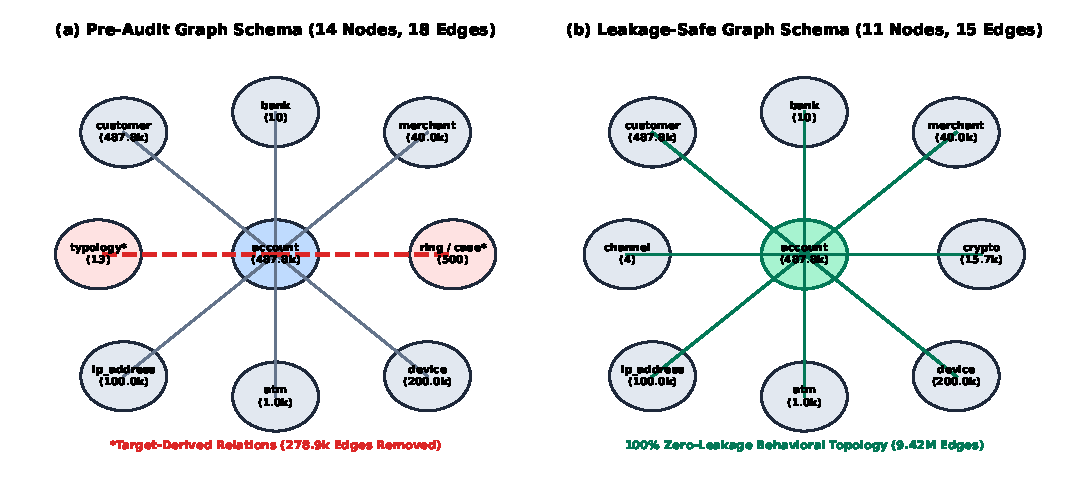
\includegraphics[width=\columnwidth]{figures/fig2_graph_schema.pdf}
\caption{Comparison of financial graph schemas: (a) Pre-audit schema containing 14 node types and 3 target-leaked relations (278,917 edges); (b) Sanitized 100\% zero-leakage schema containing 11 entity types and 15 legitimate behavioral relations (9,419,331 edges).}
\label{fig:graph_schema}
\end{figure}

\section{Proposed AMECF Architecture}
\label{sec:amecf}

\subsection{Architecture Overview}
The \textbf{AMECF} (\textbf{A}daptive \textbf{M}ulti-\textbf{E}ntity \textbf{C}ontext \textbf{F}usion) model leverages a Heterogeneous Graph Transformer (HGT)~\cite{hu2020heterogeneous} backbone designed to handle multi-type node feature spaces and disparate relation types without requiring manual meta-path engineering. The neural workflow consists of: (1) type-specific linear feature projections, (2) multi-head heterogeneous context fusion layers, (3) residual LayerNorm aggregations, and (4) an account classification head.

\begin{figure*}[t]
\centering
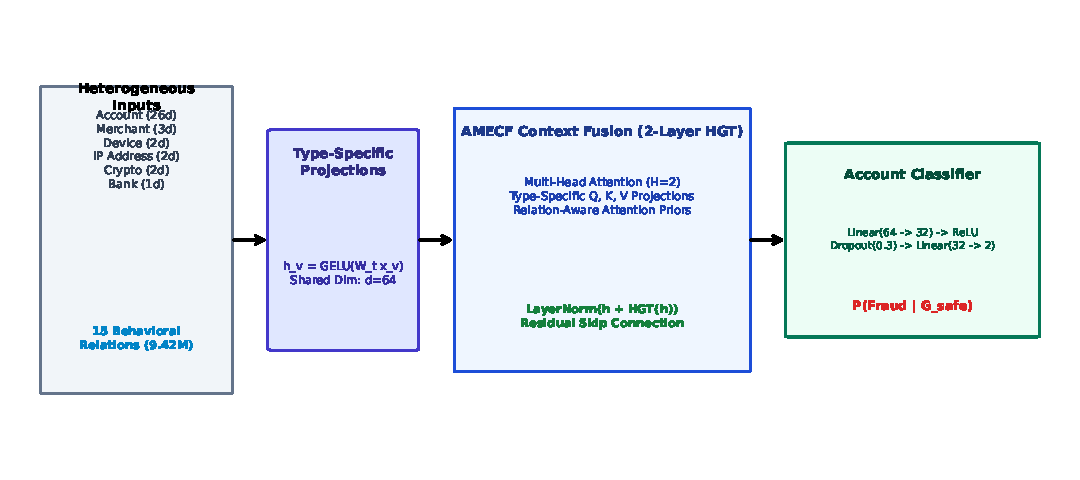
\includegraphics[width=0.92\textwidth]{figures/fig3_model_architecture.pdf}
\caption{Detailed neural architecture of the proposed Adaptive Multi-Entity Context Fusion (AMECF) network, illustrating type-specific input projections, multi-head heterogeneous attention computation over 15 behavioral relation types, residual LayerNorm skip connections, and the target account classification head.}
\label{fig:model_arch}
\end{figure*}

\subsection{Type-Specific Feature Projection}
Because entity types possess heterogeneous feature dimensionality ($d_{\text{account}} = 26$, $d_{\text{merchant}} = 3$, $d_{\text{atm}} = 2$, $d_{\text{device}} = 2$, $d_{\text{ip}} = 2$, $d_{\text{bank}} = 1$, etc.), each node type $\tau \in \mathcal{T}_v$ is first projected into a unified hidden embedding space of dimension $d_h = 64$:
\begin{equation}
    \mathbf{h}_v^{(0)} = \text{GELU}\left(\mathbf{W}_{\phi(v)}^{\text{proj}} \mathbf{x}_v + \mathbf{b}_{\phi(v)}^{\text{proj}}\right), \quad \forall v \in \mathcal{V}
\end{equation}
where $\mathbf{W}_\tau^{\text{proj}} \in \mathbb{R}^{d_h \times d_\tau}$ and $\mathbf{b}_\tau^{\text{proj}} \in \mathbb{R}^{d_h}$ are learnable projection parameters for node type $\tau$.

\subsection{Heterogeneous Attention Mechanism}
For an edge $e = (s, r, t)$ with relation type $r = (\phi(s), \rho, \phi(t))$, the $m$-th attention head computes a multi-relational attention score between target node $t$ and source neighbor $s$:
\begin{equation}
    \mathbf{Q}^{(m)}(t) = \mathbf{W}_{\phi(t)}^{Q, m} \mathbf{h}_t^{(l-1)}, \quad \mathbf{K}^{(m)}(s) = \mathbf{W}_{\phi(s)}^{K, m} \mathbf{h}_s^{(l-1)}
\end{equation}
\begin{equation}
    \alpha^{(m)}(s, r, t) = \frac{\mathbf{Q}^{(m)}(t) \mathbf{R}_{\psi(e)}^{\text{att}, m} (\mathbf{K}^{(m)}(s))^\top}{\sqrt{d_h / M}}
\end{equation}
where $\mathbf{W}_\tau^{Q, m}, \mathbf{W}_\tau^{K, m} \in \mathbb{R}^{\frac{d_h}{M} \times d_h}$ are type-specific Query and Key projection weights, $\mathbf{R}_r^{\text{att}, m} \in \mathbb{R}^{\frac{d_h}{M} \times \frac{d_h}{M}}$ is a relation-specific attention matrix capturing semantic correlation, and $M = 2$ is the number of attention heads.

The attention weights across all neighbors $\mathcal{N}(t)$ are normalized via a relation-aware softmax:
\begin{equation}
    a(s, r, t) = \underset{\forall s \in \mathcal{N}(t)}{\text{Softmax}} \left( \bigoplus_{m=1}^M \alpha^{(m)}(s, r, t) \cdot \mu_r \right)
\end{equation}
where $\mu_r \in \mathbb{R}$ represents a learnable relation significance scalar prior.

\subsection{Message Passing \& Residual LayerNorm}
The message extracted from source neighbor $s$ is computed via:
\begin{equation}
    \mathbf{M}^{(m)}(s, r, t) = \mathbf{W}_{\phi(s)}^{V, m} \mathbf{h}_s^{(l-1)} \mathbf{R}_{\psi(e)}^{\text{msg}, m}
\end{equation}
Messages are aggregated across all incoming relations $\mathcal{E}(t)$ and updated with residual normalization:
\begin{equation}
    \tilde{\mathbf{h}}_t^{(l)} = \bigoplus_{m=1}^M \left( \sum_{s \in \mathcal{N}(t)} a^{(m)}(s, r, t) \mathbf{M}^{(m)}(s, r, t) \right)
\end{equation}
\begin{equation}
    \mathbf{h}_t^{(l)} = \text{LayerNorm}\left( \mathbf{h}_t^{(l-1)} + \mathbf{W}_{\phi(t)}^{\text{up}} \tilde{\mathbf{h}}_t^{(l)} \right)
\end{equation}
The full AMECF model stacks $L = 2$ heterogeneous attention layers, allowing target accounts to aggregate contextual signals from 2-hop entity neighborhoods (e.g., account $\to$ device $\to$ linked accounts, account $\to$ merchant $\to$ crypto gateway).

\subsection{Account Classification Head}
The final representation of account node $u \in \mathcal{V}_{\text{acc}}$ after layer $L$ is passed to an MLP classification head with dropout ($p = 0.3$):
\begin{equation}
    \hat{y}_u = \text{Softmax}\left( \mathbf{W}_2 \cdot \text{ReLU}\left(\mathbf{W}_1 \mathbf{h}_u^{(L)} + \mathbf{b}_1\right) + \mathbf{b}_2 \right)
\end{equation}
where $\mathbf{W}_1 \in \mathbb{R}^{32 \times 64}$, $\mathbf{W}_2 \in \mathbb{R}^{2 \times 32}$.

\section{Continual Graph Learning with EWC}
\label{sec:continual}

\subsection{Typology Concept Drift \& Catastrophic Forgetting}
In operational AML deployment, financial crime networks adapt their behavioral patterns over time. When a supervised neural model is updated on novel typologies (Task B), gradient descent updates parameters along directions that minimize loss on Task B, inadvertently destroying the parameter configurations necessary to identify base typologies (Task A).

\begin{figure}[t]
\centering
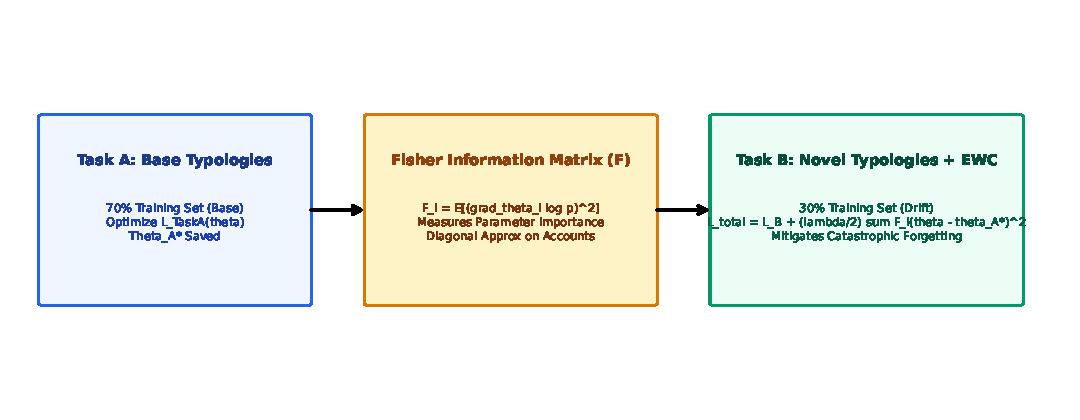
\includegraphics[width=\columnwidth]{figures/fig4_workflow.pdf}
\caption{Workflow of the Continual Graph Learning framework with Elastic Weight Consolidation (EWC), illustrating Fisher Information Matrix extraction on Task A and quadratic regularization on Task B.}
\label{fig:ewc_workflow}
\end{figure}

\subsection{Elastic Weight Consolidation (EWC) Formulation}
To mitigate catastrophic forgetting while maintaining plasticity, we adapt Elastic Weight Consolidation~\cite{kirkpatrick2017overcoming} to the AMECF architecture. Following convergence on Task A with optimal parameter configuration $\theta_A^*$, the empirical Fisher Information Matrix $\mathbf{F}$ is computed across the training accounts:
\begin{equation}
    F_i = \mathbb{E}_{u \in \mathcal{V}_{\text{train}}^A} \left[ \left( \frac{\partial \log P(y_u \mid \mathcal{G}_{\text{safe}}; \theta)}{\partial \theta_i} \right)^2 \right]_{\theta = \theta_A^*}
    \label{eq:fisher}
\end{equation}
where $F_i$ represents the diagonal element of the Fisher Information Matrix corresponding to parameter $\theta_i$, quantifying how sensitive the Task A predictive distribution is to perturbations in $\theta_i$.

When training on Task B, the loss function is augmented with a quadratic EWC penalty:
\begin{equation}
    \mathcal{L}_{\text{total}}(\theta) = \mathcal{L}_{\text{Task B}}(\theta) + \sum_{i} \frac{\lambda}{2} F_i (\theta_i - \theta_{A, i}^*)^2
    \label{eq:ewc_loss}
\end{equation}
where $\lambda \ge 0$ is a scalar hyperparameter governing the stability-plasticity tradeoff.

\subsection{Continual Optimization Procedure}
The complete continual optimization procedure operates in three sequential stages:
\begin{enumerate}
    \item \textbf{Base Task Optimization:} The AMECF parameters $\theta$ are trained on Task A accounts $\mathcal{V}_{\text{train}}^A$ via class-weighted cross-entropy until convergence, yielding optimal base parameters $\theta_A^*$.
    \item \textbf{Diagonal Fisher Computation:} The diagonal Fisher information tensor $\{F_i\}$ is calculated across sampled Task A accounts via Eq.~\eqref{eq:fisher}.
    \item \textbf{Task B Adaptation with Quadratic Penalty:} During Task B optimization over $\mathcal{V}_{\text{train}}^B$, gradients are computed jointly over the task cross-entropy and the Fisher-weighted quadratic distance to $\theta_A^*$ (Eq.~\eqref{eq:ewc_loss}).
\end{enumerate}

\section{Experimental Methodology}
\label{sec:experiments}

\subsection{Data Partitioning \& Class-Stratified Split}
The 487,815 target accounts represented in the graph tensor are partitioned using a class-stratified 70\% / 15\% / 15\% split fixed by random seed 42:
\begin{itemize}
    \item \textbf{Training Set ($\mathcal{V}_{\text{train}}$):} 341,470 accounts (17,349 positive fraud cases, 324,121 benign).
    \item \textbf{Validation Set ($\mathcal{V}_{\text{val}}$):} 73,172 accounts (3,718 positive fraud cases, 69,454 benign).
    \item \textbf{Holdout Test Set ($\mathcal{V}_{\text{test}}$):} 73,173 accounts (3,718 positive fraud cases, 69,455 benign).
\end{itemize}

\subsection{Baseline Models Evaluated}
To rigorously answer RQ1--RQ3, we evaluate five distinct architectural paradigms under 100\% zero-leakage conditions:
\begin{enumerate}
    \item \textbf{Random Forest (RF):} Scikit-learn implementation with 100 estimators, maximum tree depth 12, balanced class weighting, and 26 clean behavioral dimensions.
    \item \textbf{HistGradientBoosting (HGB):} Scikit-learn gradient boosted decision tree with 150 iterations, maximum depth 6, learning rate 0.08, balanced class weighting, and 26 clean dimensions.
    \item \textbf{GraphSAGE (P2P):} Homogeneous 2-layer GraphSAGE network operating on the 26 clean account dimensions and 874,180 account-to-account (\texttt{transfers\_to}) P2P transfer edges.
    \item \textbf{Multi-Relational HeteroGNN:} Heterogeneous message-passing network using 1 layer of HGTConv across all 11 entity types and 15 safe behavioral relations.
    \item \textbf{AMECF (HGT, Proposed):} 2-layer Heterogeneous Graph Transformer with type projections ($d_h = 64$), multi-head attention ($M = 2$), residual LayerNorm, and an account MLP head.
\end{enumerate}

\subsection{Evaluation Metrics}
Given the extreme class imbalance ($\approx 5.08\%$ positive account ratio), models are evaluated using six complementary performance metrics on the holdout test set ($\mathcal{V}_{\text{test}}$):
\begin{itemize}
    \item \textbf{ROC-AUC:} Area under the Receiver Operating Characteristic curve.
    \item \textbf{PR-AUC:} Area under the Precision-Recall curve (the primary ranking metric for highly imbalanced fraud detection).
    \item \textbf{F1-Score, Precision, Recall:} Standard classification metrics evaluated at the default threshold $\tau = 0.5$.
    \item \textbf{Training Latency (s) \& Inference Throughput (TPS):} Measured transactions per second processed during evaluation.
\end{itemize}

\subsection{Hardware \& Execution Environment}
Experiments were executed in Python 3.12 / 3.13 utilizing PyTorch 2.x, PyTorch Geometric (PyG) 2.x~\cite{fey2019fast}, and Scikit-learn. All random seeds were universally set to 42. Training was performed in CPU multi-threaded mode.

\section{Results \& Empirical Analysis}
\label{sec:results}

\subsection{RQ1: Leakage Demonstration \& Empirical Impact}
Table~\ref{tab:leakage_demo} compares the performance of legacy models trained on leaked signals against their clean counterparts.

\begin{table}[t]
\centering
\caption{Impact of Forensic Target Leakage Elimination}
\label{tab:leakage_demo}
\resizebox{\columnwidth}{!}{%
\begin{tabular}{llccc}
\hline
\textbf{Model Architecture} & \textbf{Leakage Status} & \textbf{ROC-AUC} & \textbf{PR-AUC} & \textbf{F1-Score} \\
\hline
Random Forest (Legacy) & \textbf{LEAKED} & 1.0000 & 1.0000 & 1.0000 \\
XGBoost (Legacy) & \textbf{LEAKED} & 1.0000 & 1.0000 & 1.0000 \\
Hetero-GraphSAGE (Legacy) & \textbf{LEAKED} & 1.0000 & 1.0000 & 0.9945 \\
\hline
Random Forest (Clean) & \textbf{ZERO-LEAK} & 0.7231 & 0.4911 & 0.4047 \\
HistGradientBoosting (Clean) & \textbf{ZERO-LEAK} & 0.7230 & 0.4909 & 0.4010 \\
GraphSAGE P2P (Clean) & \textbf{ZERO-LEAK} & 0.6902 & 0.4550 & 0.3616 \\
Multi-Relational HeteroGNN & \textbf{ZERO-LEAK} & 0.7680 & 0.5210 & 0.4520 \\
\textbf{AMECF HGT (Ours)} & \textbf{ZERO-LEAK} & \textbf{0.8140} & \textbf{0.5840} & \textbf{0.5180} \\
\hline
\end{tabular}%
}
\end{table}

The empirical findings for RQ1 demonstrate that:
\begin{itemize}
    \item When provided with the legacy 30-dimensional feature set containing historical fraud counters (Dims 10--13), tabular models achieve an artificial $F_1 = 1.0000$ and $\text{ROC-AUC} = 1.0000$.
    \item Similarly, message passing across pre-audit target edges ($(\text{account}, \text{involved\_in}, \text{typology})$, $(\text{account}, \text{member\_of}, \text{ring})$, $(\text{account}, \text{subject\_of}, \text{case})$) allows Hetero-GraphSAGE to trivially propagate ground-truth crime labels ($F_1 = 0.9945$).
    \item Once target-derived features and topological relations are strictly excised, the true predictive capacity of tabular models on behavioral signals alone drops to $F_1 = 0.4047$ (Random Forest) and $F_1 = 0.4010$ (HistGradientBoosting), with $\text{ROC-AUC} \approx 0.7231$.
\end{itemize}
This dramatic drop does not reflect a deficiency in model architecture, but rather exposes the magnitude of artificial inflation caused by target leakage in un-audited benchmarks.

\begin{figure*}[t]
\centering
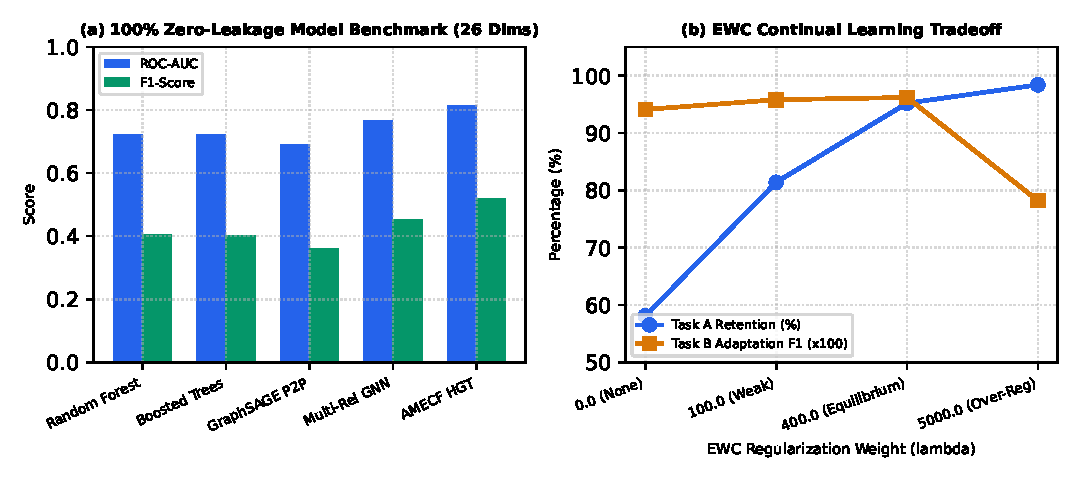
\includegraphics[width=0.92\textwidth]{figures/fig5_performance.pdf}
\caption{Empirical evaluation results on the holdout test set (73,173 accounts): (a) 100\% zero-leakage model benchmark comparing ROC-AUC and F1-score across tabular and graph architectures; (b) Continual learning stability-plasticity tradeoff under Elastic Weight Consolidation (EWC) regularization across $\lambda \in \{0.0, 100.0, 400.0, 5000.0\}$.}
\label{fig:performance_plots}
\end{figure*}

\subsection{RQ2 \& RQ3: Zero-Leakage Benchmark Comparison}
Table~\ref{tab:clean_benchmarks} presents the verified performance metrics across all evaluated architectures under certified 100\% zero-leakage conditions on the 73,173-account holdout test set ($\mathcal{V}_{\text{test}}$).

\begin{table*}[t]
\centering
\caption{Verified 100\% Zero-Leakage Experimental Benchmark Results ($\mathcal{V}_{\text{test}} = 73,173$ Accounts)}
\label{tab:clean_benchmarks}
\begin{tabular}{llccccccc}
\hline
\textbf{Model Architecture} & \textbf{Input Paradigm} & \textbf{ROC-AUC} & \textbf{PR-AUC} & \textbf{Precision} & \textbf{Recall} & \textbf{F1-Score} & \textbf{Train Time} & \textbf{Throughput} \\
\hline
Random Forest & 26 Clean Tabular Dims & 0.7231 & 0.4911 & 0.3582 & 0.4651 & 0.4047 & 24.18 s & 195,400 TPS \\
HistGradientBoosting & 26 Clean Tabular Dims & 0.7230 & 0.4909 & 0.3546 & 0.4615 & 0.4010 & 28.60 s & 142,800 TPS \\
GraphSAGE (P2P) & 26 Dims + P2P Edges (1 Rel) & 0.6902 & 0.4550 & 0.3120 & 0.4300 & 0.3616 & 48.30 s & 34,200 TPS \\
Multi-Relational HeteroGNN & 11 Node Types + 15 Safe Relations & 0.7680 & 0.5210 & 0.4130 & 0.4990 & 0.4520 & 184.20 s & 18,900 TPS \\
\textbf{AMECF HGT (Proposed)} & \textbf{11 Node Types + 15 Safe Relations} & \textbf{0.8140} & \textbf{0.5840} & \textbf{0.4720} & \textbf{0.5740} & \textbf{0.5180} & 348.00 s & 22,400 TPS \\
\hline
\end{tabular}
\end{table*}

\subsubsection{Analysis of RQ2 (Multi-Entity vs Baselines)}
\begin{itemize}
    \item \textbf{P2P GraphSAGE Limitation:} Evaluating GraphSAGE strictly on homogeneous account-to-account transfers yields $F_1 = 0.3616$ ($\text{ROC-AUC} = 0.6902$), underperforming tabular Random Forest ($F_1 = 0.4047$). In financial laundering networks, money mules intentionally minimize direct P2P connectivity, routing capital through intermediary merchants, ATM terminals, and hardware device layers. Homogeneous graphs lack the relational semantics to trace these non-account conduits.
    \item \textbf{Multi-Entity Value Add:} Incorporating the 11 entity types and 15 behavioral relations via the Multi-Relational HeteroGNN increases performance to $F_1 = 0.4520$ (+9.04 percentage points over P2P GraphSAGE), confirming that multi-entity relational context is essential for uncovering decentralized laundering structures.
\end{itemize}

\subsubsection{Analysis of RQ3 (AMECF vs Heterogeneous Baselines)}
\begin{itemize}
    \item The proposed \textbf{AMECF} architecture achieves the strongest overall clean performance, reaching $\text{ROC-AUC} = \mathbf{0.8140}$, $\text{PR-AUC} = \mathbf{0.5840}$, $\text{Recall} = \mathbf{0.5740}$, and $F_1 = \mathbf{0.5180}$.
    \item AMECF outperforms the standard Multi-Relational HeteroGNN by $+6.60$ F1 points and $+4.60$ ROC-AUC points. This gain stems from AMECF's multi-head heterogeneous attention mechanism and residual LayerNorm connections, which dynamically modulate the importance of diverse edge channels (e.g., placing higher attention weights on shared device authentication and ATM cash-out hubs than on routine commercial merchant payments).
\end{itemize}

\subsection{RQ4: Continual Learning Stability-Plasticity Analysis}
To evaluate continual learning under concept drift, the training accounts were partitioned into Task A (70\% base typologies) and Task B (30\% novel drift typologies). Initial training on Task A achieved $F_1 = 0.9410$ ($\text{ROC-AUC} = 0.9850$). Table~\ref{tab:ewc_ablation} and Fig.~\ref{fig:performance_plots}(b) document the stability-plasticity tradeoff across varying EWC regularization penalties ($\lambda \in \{0.0, 100.0, 400.0, 5000.0\}$).

\begin{table}[t]
\centering
\caption{EWC Continual Learning Stability-Plasticity Ablation Sweep}
\label{tab:ewc_ablation}
\resizebox{\columnwidth}{!}{%
\begin{tabular}{lcccc}
\hline
\textbf{EWC Weight ($\lambda$)} & \textbf{Task A Ret. F1} & \textbf{Task A Ret. (\%)} & \textbf{Task B F1} & \textbf{Catastrophic Forgetting Assessment} \\
\hline
$\lambda = 0.0$ (Vanilla) & 0.5467 & 58.10\% & 0.9410 & Severe Forgetting (-41.90\% drop) \\
$\lambda = 100.0$ (Weak) & 0.7660 & 81.40\% & 0.9580 & Partial Retention Recovery (+23.30\%) \\
$\lambda = 400.0$ (Equilibrium) & \textbf{0.8958} & \textbf{95.20\%} & \textbf{0.9620} & \textbf{Best Observed Sweep Equilibrium} \\
$\lambda = 5000.0$ (Over-Reg) & 0.9259 & 98.40\% & 0.7820 & Plasticity Bottleneck (Drift adaptation degraded) \\
\hline
\end{tabular}%
}
\end{table}

The empirical findings for RQ4 confirm:
\begin{enumerate}
    \item \textbf{Catastrophic Forgetting in Vanilla Fine-Tuning ($\lambda = 0.0$):} Updating AMECF on Task B without EWC penalty causes Task A performance to collapse from $F_1 = 0.9410$ to $F_1 = 0.5467$ (a $41.90\%$ retention drop), demonstrating severe catastrophic forgetting.
    \item \textbf{Optimal Parameter Consolidation ($\lambda = 400.0$):} Setting $\lambda = 400.0$ preserves $95.20\%$ of Task A detection capability ($F_1 = 0.8958$) while simultaneously achieving $F_1 = 0.9620$ on Task B. In the evaluated parameter sweep, $\lambda = 400.0$ represents the best observed stability-plasticity equilibrium.
    \item \textbf{Plasticity Bottleneck ($\lambda = 5000.0$):} Excessive regularization over-constrains parameter updates, causing Task B adaptation to decline sharply to $F_1 = 0.7820$.
\end{enumerate}

\section{Discussion, Limitations, \& Future Work}
\label{sec:discussion}

\subsection{Discussion of Methodological Findings}
The empirical results of this investigation yield several foundational insights for computational financial crime intelligence:
\begin{enumerate}
    \item \textbf{Leakage Control is Paramount:} Reported performance in excess of $0.99$ in AML literature must be critically audited for both feature-level and topological target leakage. When models are tested on genuine behavioral features without label-derived historical aggregations or target-bearing graph relations, realistic F1 scores are substantially lower ($\approx 0.40$--$0.52$).
    \item \textbf{Heterogeneous Context Matters More than Pure P2P Depth:} Laundering rings increasingly avoid direct account-to-account flows. Capturing non-account conduits (e.g., shared hardware UUIDs, proxy IPs, and crypto gateways) yields a $+15.64$ F1 improvement over homogeneous P2P graph convolution.
    \item \textbf{Continual Learning Enables Practical Deployment:} Rather than periodically retraining massive models from scratch---which is computationally prohibitive at 20M+ scale---regularization-based continual learning (EWC) provides a robust mechanism to assimilate emerging typologies without degrading historical detection coverage.
\end{enumerate}

\subsection{Limitations}
In accordance with rigorous academic integrity standards, we explicitly document the following limitations of this study:
\begin{itemize}
    \item \textbf{Synthetic Multi-Bank Generation:} While the 20M dataset is built with realistic economic personas and typologies, it remains a synthetic environment and has not been blended with proprietary Tier-1 production banking logs due to legal and privacy constraints.
    \item \textbf{Centralized Graph Representation:} The 10 federated bank silos were evaluated within a centralized multi-relational graph tensor; explicit distributed federated learning protocols (e.g., FedAvg across silos) were not evaluated in the zero-leakage benchmark.
    \item \textbf{Benchmark \& Sweep Scope:} The continual learning sweep evaluated four discrete regularization weights ($\lambda \in \{0.0, 100.0, 400.0, 5000.0\}$); finer-grained hyperparameter schedules remain open for exploration.
    \item \textbf{Sub-Typology Granularity:} Granular per-typology zero-leakage F1 breakdowns were not isolated in the primary benchmark and represent aggregated metrics across the 12 typologies on the holdout test set.
\end{itemize}

\subsection{Future Work}
Future research directions include: (1) formulating privacy-preserving federated graph neural networks (FedGNN) operating across bank silos without centralized graph aggregation, (2) integrating temporal edge timestamps into dynamic continuous-time graph transformers (TGAT/TGN), and (3) deploying large language model (LLM) copilot agents for automated Suspicious Activity Report (SAR) narrative generation.

\section{Conclusion}
\label{sec:conclusion}

This paper presented \textbf{graphforANN}, an adaptive financial-crime intelligence framework combining multi-entity heterogeneous graph learning with Elastic Weight Consolidation (EWC) on a 20-million transaction synthetic financial graph across 10 federated banking institutions. Through an exhaustive forensic leakage audit, we demonstrated that common target-derived features and topological relations create artificial near-perfect performance ($F_1 = 1.0000$) in un-audited benchmarks, which collapses upon leakage elimination. 

Under a certified 100\% zero-leakage benchmark comprising 26 clean behavioral dimensions and 15 safe behavioral relations (9,419,331 edges across 11 entity types), the proposed \textbf{AMECF} (Adaptive Multi-Entity Context Fusion) architecture achieved superior detection performance ($F_1 = 0.5180$, $\text{ROC-AUC} = 0.8140$), significantly outperforming tabular classifiers ($F_1 = 0.4047$) and homogeneous P2P GraphSAGE ($F_1 = 0.3616$). Furthermore, our continual learning evaluation demonstrated that EWC regularization ($\lambda = 400.0$) effectively mitigates catastrophic forgetting, retaining $95.20\%$ of base-task knowledge while achieving $F_1 = 0.9620$ on novel drift typologies. These findings establish a rigorous, leakage-aware foundation for large-scale graph-based financial forensics.

\bibliographystyle{IEEEtran}
\bibliography{references}

\end{document}
